\documentclass[12pt,addpoints,answers]{evalua}
\grado{2$^\circ$ de Secundaria}
\cicloescolar{2023-2024}
\materia{Matemáticas 2}
\unidad{1}
\title{Examen de la Unidad}
\aprendizajes{
      \item Resuelve problemas de multiplicación y división con números enteros, fracciones y decimales positivos y negativos.
      \item Resuelve problemas de potencias con exponente entero y aproxima raíces cuadradas.
      \item Resuelve problemas que impliquen el uso de la notación científica.
      \item Calcula porcentajes de cantidades.
}
\author{Prof.: Julio César Melchor Pinto}
\begin{document}
\begin{questions}
      \section*{\ifprintanswers{Cálculos numéricos}\else{}\fi}

      \question[10] Realiza las siguientes operaciones de \textit{cálculo numérico}:
      \begin{parts}
            \begin{multicols}{2}
                  \subsection*{\ifprintanswers{Suma de números}\else{}\fi}
                  \part $849.332+242.25+469.381=$ \fillin[$1560.963$][0in]
                  \subsection*{\ifprintanswers{Resta de números}\else{}\fi}
                  \part $4934-451-682=$ \fillin[$3801$][0in]
                  \subsection*{\ifprintanswers{Multiplicación de números}\else{}\fi}
                  \part $19.3\times6.27=$ \fillin[$121.011$][0in]
                  \subsection*{\ifprintanswers{División de números}\else{}\fi}
                  \part $922\divisionsymbol1.2=$ \fillin[$768.333$][0in]
            \end{multicols}
            \subsection*{\ifprintanswers{Resolución de problemas}\else{}\fi}
            \part Entre José y su hermano están arreglando el jardín de su casa. José arregló $\dfrac{3}{8}$ del jardín y su hermano $\dfrac{1}{4}$. ¿Qué parte del jardín han arreglado?
            \begin{solutionbox}{3cm}
                  \[\dfrac{3}{8}+\dfrac{1}{4}=\dfrac{3}{8}+\dfrac{2}{8}=\dfrac{5}{8}\]
            \end{solutionbox}
      \end{parts}

      \newpage

      \section*{\ifprintanswers{Números negativos}\else{}\fi}
      \subsection*{\ifprintanswers{Ubicación en la recta numérica}\else{}\fi}
      \question[4] Escribe el número que representa el punto indicado en la recta numérica de cada uno de los siguientes incisos.

      \begin{multicols}{2}
            \begin{parts}
                  \part 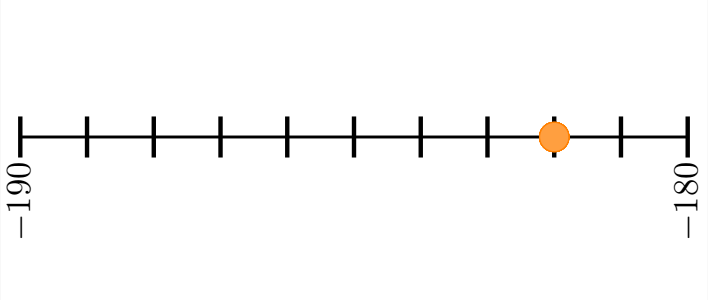
\includegraphics[width=150px]{../images/recta_num_-182.png} \\[-0.5em]   \fillin[$-182$][1.5in]
                  \part 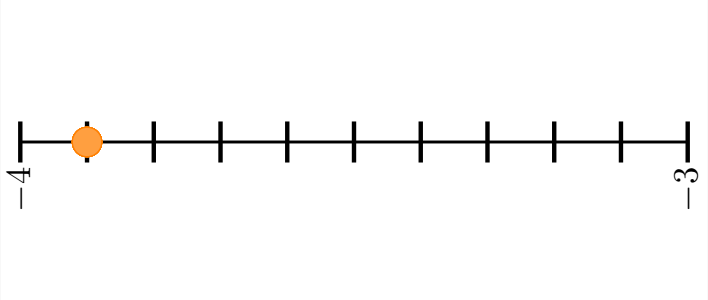
\includegraphics[width=150px]{../images/recta_num_-3.9.png} \\[-0.5em]  \fillin[$-3.9$][1.5in]
            \end{parts}
      \end{multicols}

      \subsection*{\ifprintanswers{Comparación de negativos}\else{}\fi}
      \question[4] Escribe sobre la línea el símbolo de mayor que ($>$), menor que ($<$), o igual ($=$) según corresponda.

      \begin{multicols}{2}
            \begin{parts}
                  \part $-182$ \fillin[$>$][0.5in] $-189$
                  \part $-97$ \fillin[$<$][0.5in] $-96.2$
            \end{parts}
      \end{multicols}

      \subsection*{\ifprintanswers{Suma y resta con negativos }\else{}\fi}
      \question[4] Realiza las siguientes sumas y restas con números negativos:

      \begin{multicols}{2}
            \begin{parts}
                  \part $-223+67=$ \fillin[$-156$][0in]
                  \part $(16)-(-14)=$ \fillin[$30$][0in]
            \end{parts}
      \end{multicols}

      \subsection*{\ifprintanswers{Multiplicación y división con negativos}\else{}\fi}
      \question[4] Realiza las siguientes multiplicaciones y divisiones con números negativos:
      \begin{multicols}{2}
            \begin{parts}
                  \part $(31)\divisionsymbol (-62)=$ \fillin[$-\dfrac{1}{2}$][0in]
                  \part $(-15)(-14)=$ \fillin[$210$][0in]
            \end{parts}
      \end{multicols}

      \subsection*{\ifprintanswers{Potencias con números negativos}\else{}\fi}
      \question[4] Realiza las siguientes potencias de números negativos:
      \begin{multicols}{2}
            \begin{parts}
                  \part $-7^2=$ \fillin[$-49$][0in]
                  \part $(-5)^3=$ \fillin[$-125$][0in]
            \end{parts}
      \end{multicols}


      \section*{\ifprintanswers{Exponentes y notación científica}\else{}\fi}
      \question[6] Realiza las siguientes operaciones con exponentes:
      \begin{multicols}{3}
            \begin{parts}
                  \subsection*{\ifprintanswers{Suma de exponentes}\else{}\fi}
                  \part $(-5a^4)(-3a^2)=$ \fillin[$15a^6$][0in]
                  \subsection*{\ifprintanswers{Resta de exponentes}\else{}\fi}
                  \part $\dfrac{x^{13}y^{18}z^{4}}{x^{11}y^{9}z^{4}}=$ \fillin[$x^2y^9$][0in]
                  \subsection*{\ifprintanswers{Multiplicación de exponentes}\else{}\fi}
                  \part $(a^3b^2c^4)^3=$ \fillin[$a^9b^6c^{12}$][0in]
            \end{parts}
      \end{multicols}

      \newpage
      \subsection*{\ifprintanswers{Notación científica}\else{}\fi}
      \question[4] Escribe en notación científica los siguientes números:
      \begin{multicols}{2}
            \begin{parts}
                  \part $0.0000005=$ \fillin[$ 5\times10^{-7}$][0in]
                  \part $9200000000=$ \fillin[$ 9.2\times10^9$][0in]            \end{parts}
      \end{multicols}
      \question[4] Escribe en notación decimal los siguientes números:
      \begin{multicols}{2}
            \begin{parts}
                  \part $6.7 \times 10^{4}=$ \fillin[$67000$][0in]
                  \part $7.2 \times 10^{-6}=$ \fillin[$0.0000072$][0in]            \end{parts}
      \end{multicols}

      \section*{\ifprintanswers{Plano cartesiano y la recta}\else{}\fi}
      \subsection*{\ifprintanswers{Ubicación en el plano cartesiano}\else{}\fi}
      \question[10] Escribe las coordenadas de los puntos indicados en el plano cartesiano de cada uno de los siguientes incisos.
      \begin{multicols}{2}
            \begin{parts}
                  \part Coordenadas del punto A = \fillin[$(1,5)$][0in]
                  \part Coordenadas del punto B = \fillin[$(-3,6)$][0in]
                  \part Coordenadas del punto C = \fillin[$(5,-3)$][0in]
                  \part Coordenadas del punto D = \fillin[$(-5,0$][0in]
                  \part Coordenadas del punto E = \fillin[$(0,-7)$][0in]
            \end{parts}
            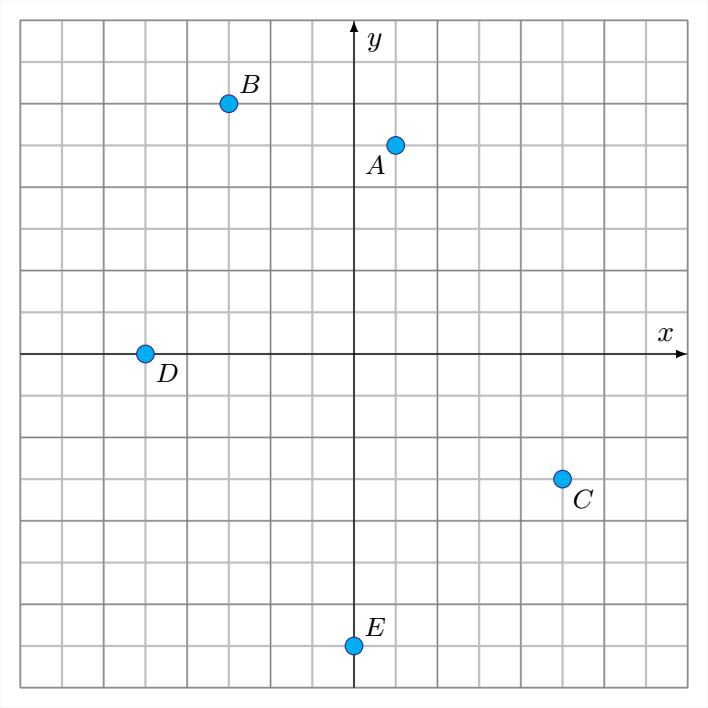
\includegraphics[width=0.8\linewidth]{../images/imagen_plano01.png}
      \end{multicols}

      \subsection*{\ifprintanswers{Cuadrantes en el plano cartesiano}\else{}\fi}
      \question[2] Escribe el número del cuadrante en el que se encuentra el punto C en el plano cartesiano: \fillin[4 cuad.][1in]

      \newpage
      \subsection*{\ifprintanswers{Pendiente de una recta}\else{}\fi}
      \question[8] Selecciona la opcion que corresponde a la pendiente de la recta en cada uno de los siguientes incisos:
      \begin{multicols}{2}
            \begin{parts}
                  \part
                  \begin{minipage}{0.6\linewidth}
                        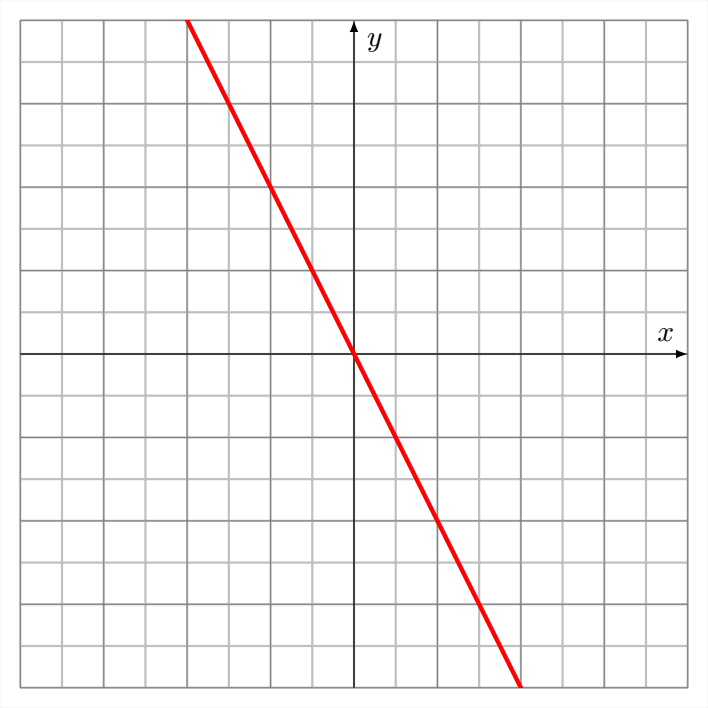
\includegraphics[width=\linewidth]{../images/plano_cart_rect_-2x.png}
                  \end{minipage}%
                  \begin{minipage}{0.5\linewidth}
                        \begin{choices}
                              \choice Positiva
                              \CorrectChoice Negativa
                              \choice Cero
                              \choice Indefinida
                        \end{choices}
                  \end{minipage}

                  \part
                  \begin{minipage}{0.6\linewidth}
                        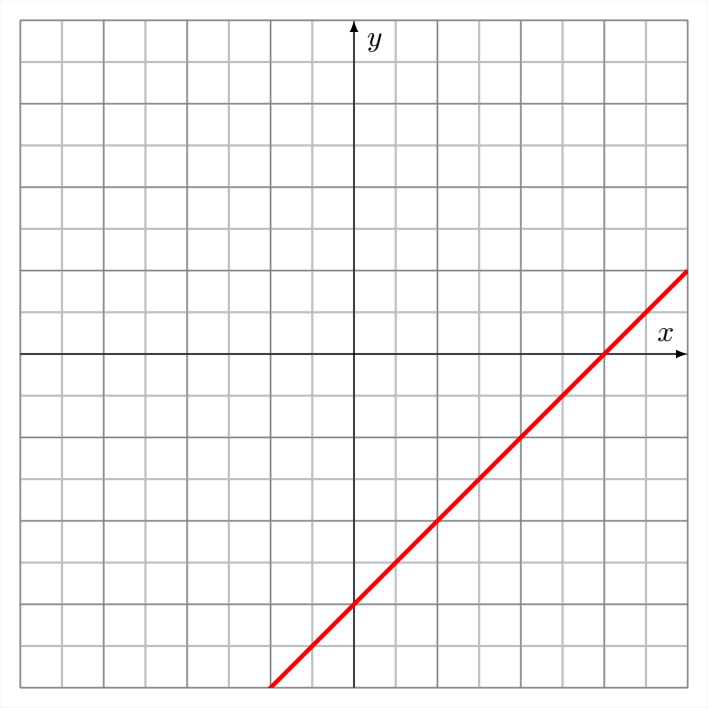
\includegraphics[width=\linewidth]{../images/plano_cart_rect_x-6.png}
                  \end{minipage}%
                  \begin{minipage}{0.5\linewidth}
                        \begin{choices}
                              \CorrectChoice Positiva
                              \choice Negativa
                              \choice Cero
                              \choice Indefinida
                        \end{choices}
                  \end{minipage}

                  \part
                  \begin{minipage}{0.6\linewidth}
                        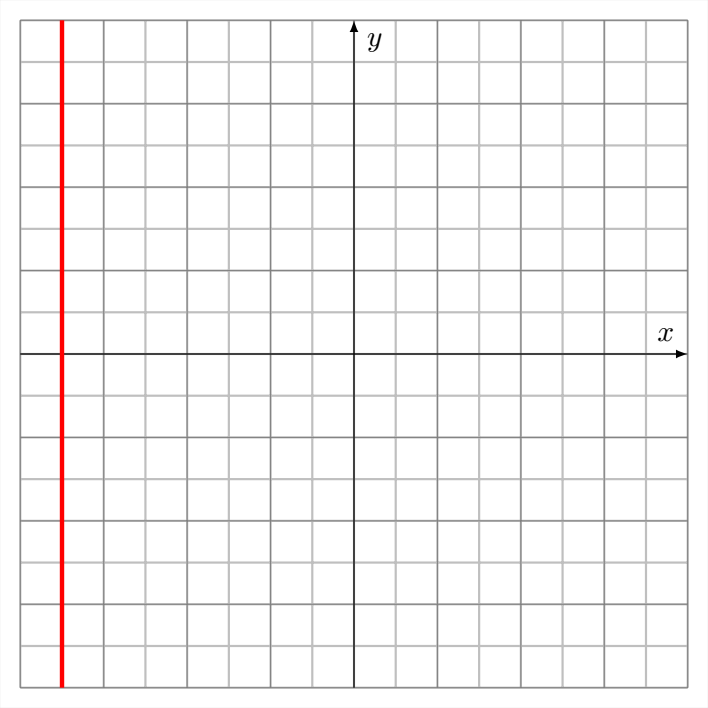
\includegraphics[width=\linewidth]{../images/plano_cart_rect_inf.png}
                  \end{minipage}%
                  \begin{minipage}{0.5\linewidth}
                        \begin{choices}
                              \choice Positiva
                              \choice Negativa
                              \choice Cero
                              \CorrectChoice Indefinida
                        \end{choices}
                  \end{minipage}

                  \part
                  \begin{minipage}{0.6\linewidth}
                        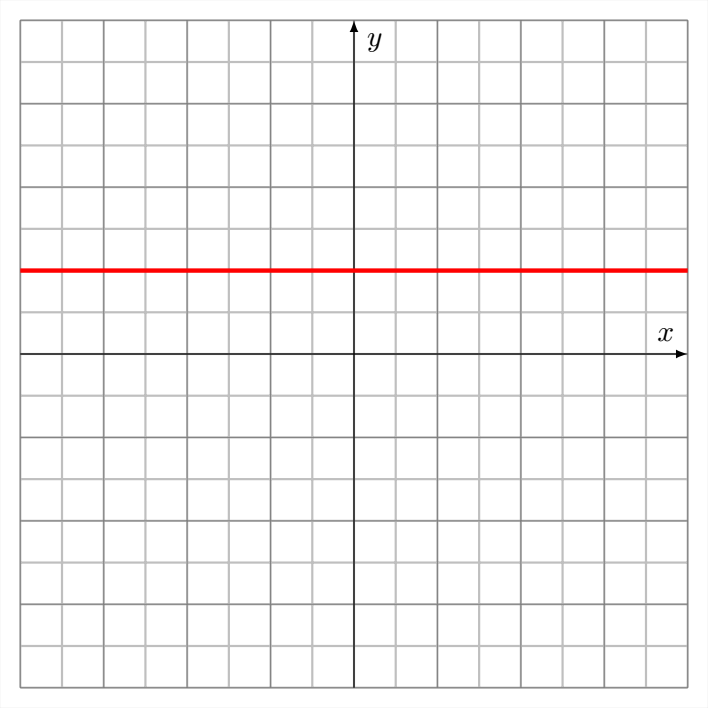
\includegraphics[width=\linewidth]{../images/plano_cart_rect_0.png}
                  \end{minipage}%
                  \begin{minipage}{0.5\linewidth}
                        \begin{choices}
                              \choice Positiva
                              \choice Negativa
                              \CorrectChoice Cero
                              \choice Indefinida
                        \end{choices}
                  \end{minipage}
            \end{parts}
      \end{multicols}
      \subsection*{\ifprintanswers{Pendiente y ordenada}\else{}\fi}
      \question[8] Identifica la pendiente y ordenada de las siguientes rectas:
      \begin{multicols}{2}
            \begin{parts}
                  \part $y=-2x+1$ \\[1em]
                  Pendiente = \fillin[$-2$][0in]\\[0.5em]
                  Ordenada = \fillin[$1$][0in]

                  \part $y=-\dfrac{2}{3}x-5$ \\[1em]
                  Pendiente = \fillin[$-\dfrac{2}{3}$][0in]\\[0.5em]
                  Ordenada = \fillin[$-5$][0in]

            \end{parts}
      \end{multicols}


      \newpage
      \subsection*{\ifprintanswers{Ecuación de una recta}\else{}\fi}
      \question[4] Escribe la ecuación de cada una de las rectas en los siguientes planos cartesianos:
      \begin{multicols}{2}
            \begin{parts}
                  \part
                  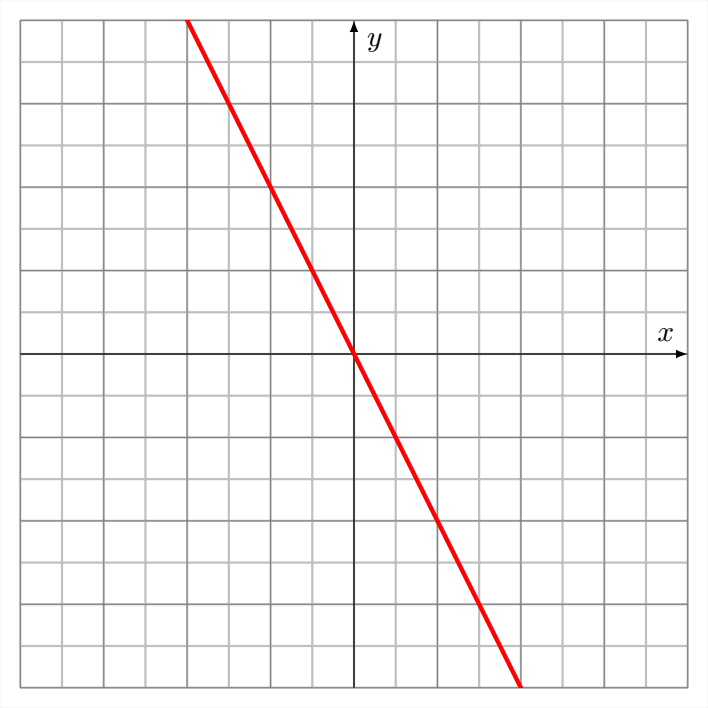
\includegraphics[width=.8\linewidth]{../images/plano_cart_rect_-2x.png}\\
                  \fillin[$y=-2x$][2in]

                  \part
                  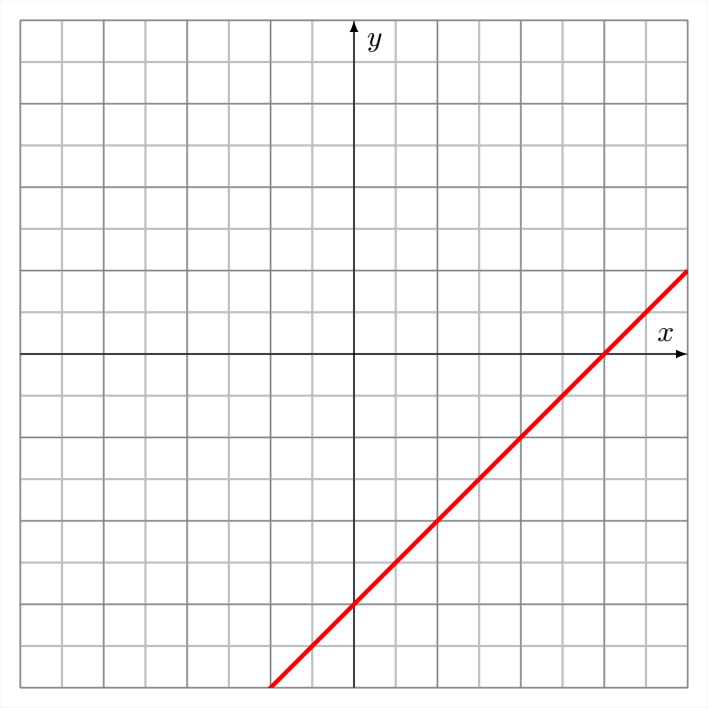
\includegraphics[width=.8\linewidth]{../images/plano_cart_rect_x-6.png}\\
                  \fillin[$y=x-6$][2in]
            \end{parts}
      \end{multicols}

      \section*{\ifprintanswers{Porcentajes}\else{}\fi}
      \subsection*{\ifprintanswers{Porcentajes a decimal}\else{}\fi}

      \question[4] Escribe el número decimal que representa cada porcentaje:

      \begin{multicols}{2}
            \begin{parts}
                  \part Convierte 401\% a un número decimal. \fillin[$0.229$][0in]
                  \part Convierte 6\% a un número decimal. \fillin[$0.062$][0in]
            \end{parts}
      \end{multicols}

      \subsection*{\ifprintanswers{Decimal a porcentaje}\else{}\fi}
      \question[4] Escribe el porcentaje que representa cada número decimal:

      \begin{multicols}{2}
            \begin{parts}
                  \part Expresa 1.44 como un porcentaje. \fillin[$144\%$][0in]
                  \part Expresa 0.092 como un porcentaje. \fillin[$9.2\%$][0in]
            \end{parts}
      \end{multicols}


      \subsection*{\ifprintanswers{Porcentaje de cantidades}\else{}\fi}
      \question[8] Calcula los porcentajes de cada una de las siguientes cantidades:
      \begin{multicols}{2}
            \begin{parts}
                  \part ¿Cuál es el 225\% de 600?
                  \begin{solutionbox}{1.5cm}
                        \[\dfrac{600\times 225\%}{100\%}=1350\]
                  \end{solutionbox}

                  \part Si se sabe que 30 es el 6\% de cierta cantidad, ¿cuál es esta cantidad?
                  \begin{solutionbox}{1.5cm}
                        \[\dfrac{30\times 100\%}{6\%}=500\]
                  \end{solutionbox}

                  \part ¿Cuál es el 23\% de 59?
                  \begin{solutionbox}{1.5cm}
                        \[\dfrac{59\times 23\%}{100\%}=13.57\]
                  \end{solutionbox}

                  \part Si se sabe que 40 es el 250\% de cierta cantidad, ¿cuál es esta cantidad?
                  \begin{solutionbox}{1.5cm}
                        \[\dfrac{40\times 100\%}{250\%}=16\]
                  \end{solutionbox}
            \end{parts}
      \end{multicols}

      \subsection*{\ifprintanswers{Resolución de problemas}\else{}\fi}
      \question[8] Resuelve los siguientes problemas:
      \begin{parts}
            \part El costo de una camisa es de \$800 pesos, si se les hace un descuento del 20\%, ¿cuánto pagaré en total por la camisa?
            \begin{solutionbox}{2cm}
                  \[\$800\times 20\%=\$160\]
                  \[\$800-\$160=\$640\]
            \end{solutionbox}

            \part El 24\% de los habitantes de un pueblo tienen menos de 30 años. ¿Cuántos habitantes tiene el pueblo si hay 120 jóvenes menores de 30 años?
            \begin{solutionbox}{2cm}
                  \[\dfrac{120\times 100\%}{24\%}=500\]
            \end{solutionbox}
      \end{parts}
\end{questions}
\end{document}